\section{Phase 3: High Fidelity Prototype}
We used the insights generated in the first two phases to design a fully immersive StoAR prototype for use in head-mounted displays. Because we did not have access to a retail testing environment, we simulated a retail display in virtual reality based on configurations found in a local retail outlet. We then added an augmented reality interface to the simulation to provide review and price information (Fig. \ref{figures:HiFiScreenshots}).\todo{briefly describe the important pieces informed by the low-fi study. MW: Hmm.. It seems redundant now that the Phase 2 section is properly concluded.} While our use of a VR store simulation removes immediate access to real life products found in a real store, the fully immersive environment allowed us to closely control the relationship between the prototype AR interfaces and simulated products. %and reduced the environmental complexity to allow participants to focus solely on the prototype implementation. 

We recruited 20 participants from a local research expo to evaluate our prototype. Participants first freely navigated the virtual representation of a store augmented with static content containing information about each device. After navigating the scene, participants completed a short survey that asked for their perceptions of the prototype's usability, potential impact on decision-making, utility of individual design components, perceived trade-offs compared to existing technologies, and potential limitations of the approach. They also provided feedback on additional applications where they envisioned using mixed reality experiences for decision making. As with the initial online survey, we analyzed the qualitative feedback provided by users by clustering their responses into common themes. 

\begin{marginfigure}
	\begin{minipage}{\marginparwidth}
		\centering
		\subfloat[][]{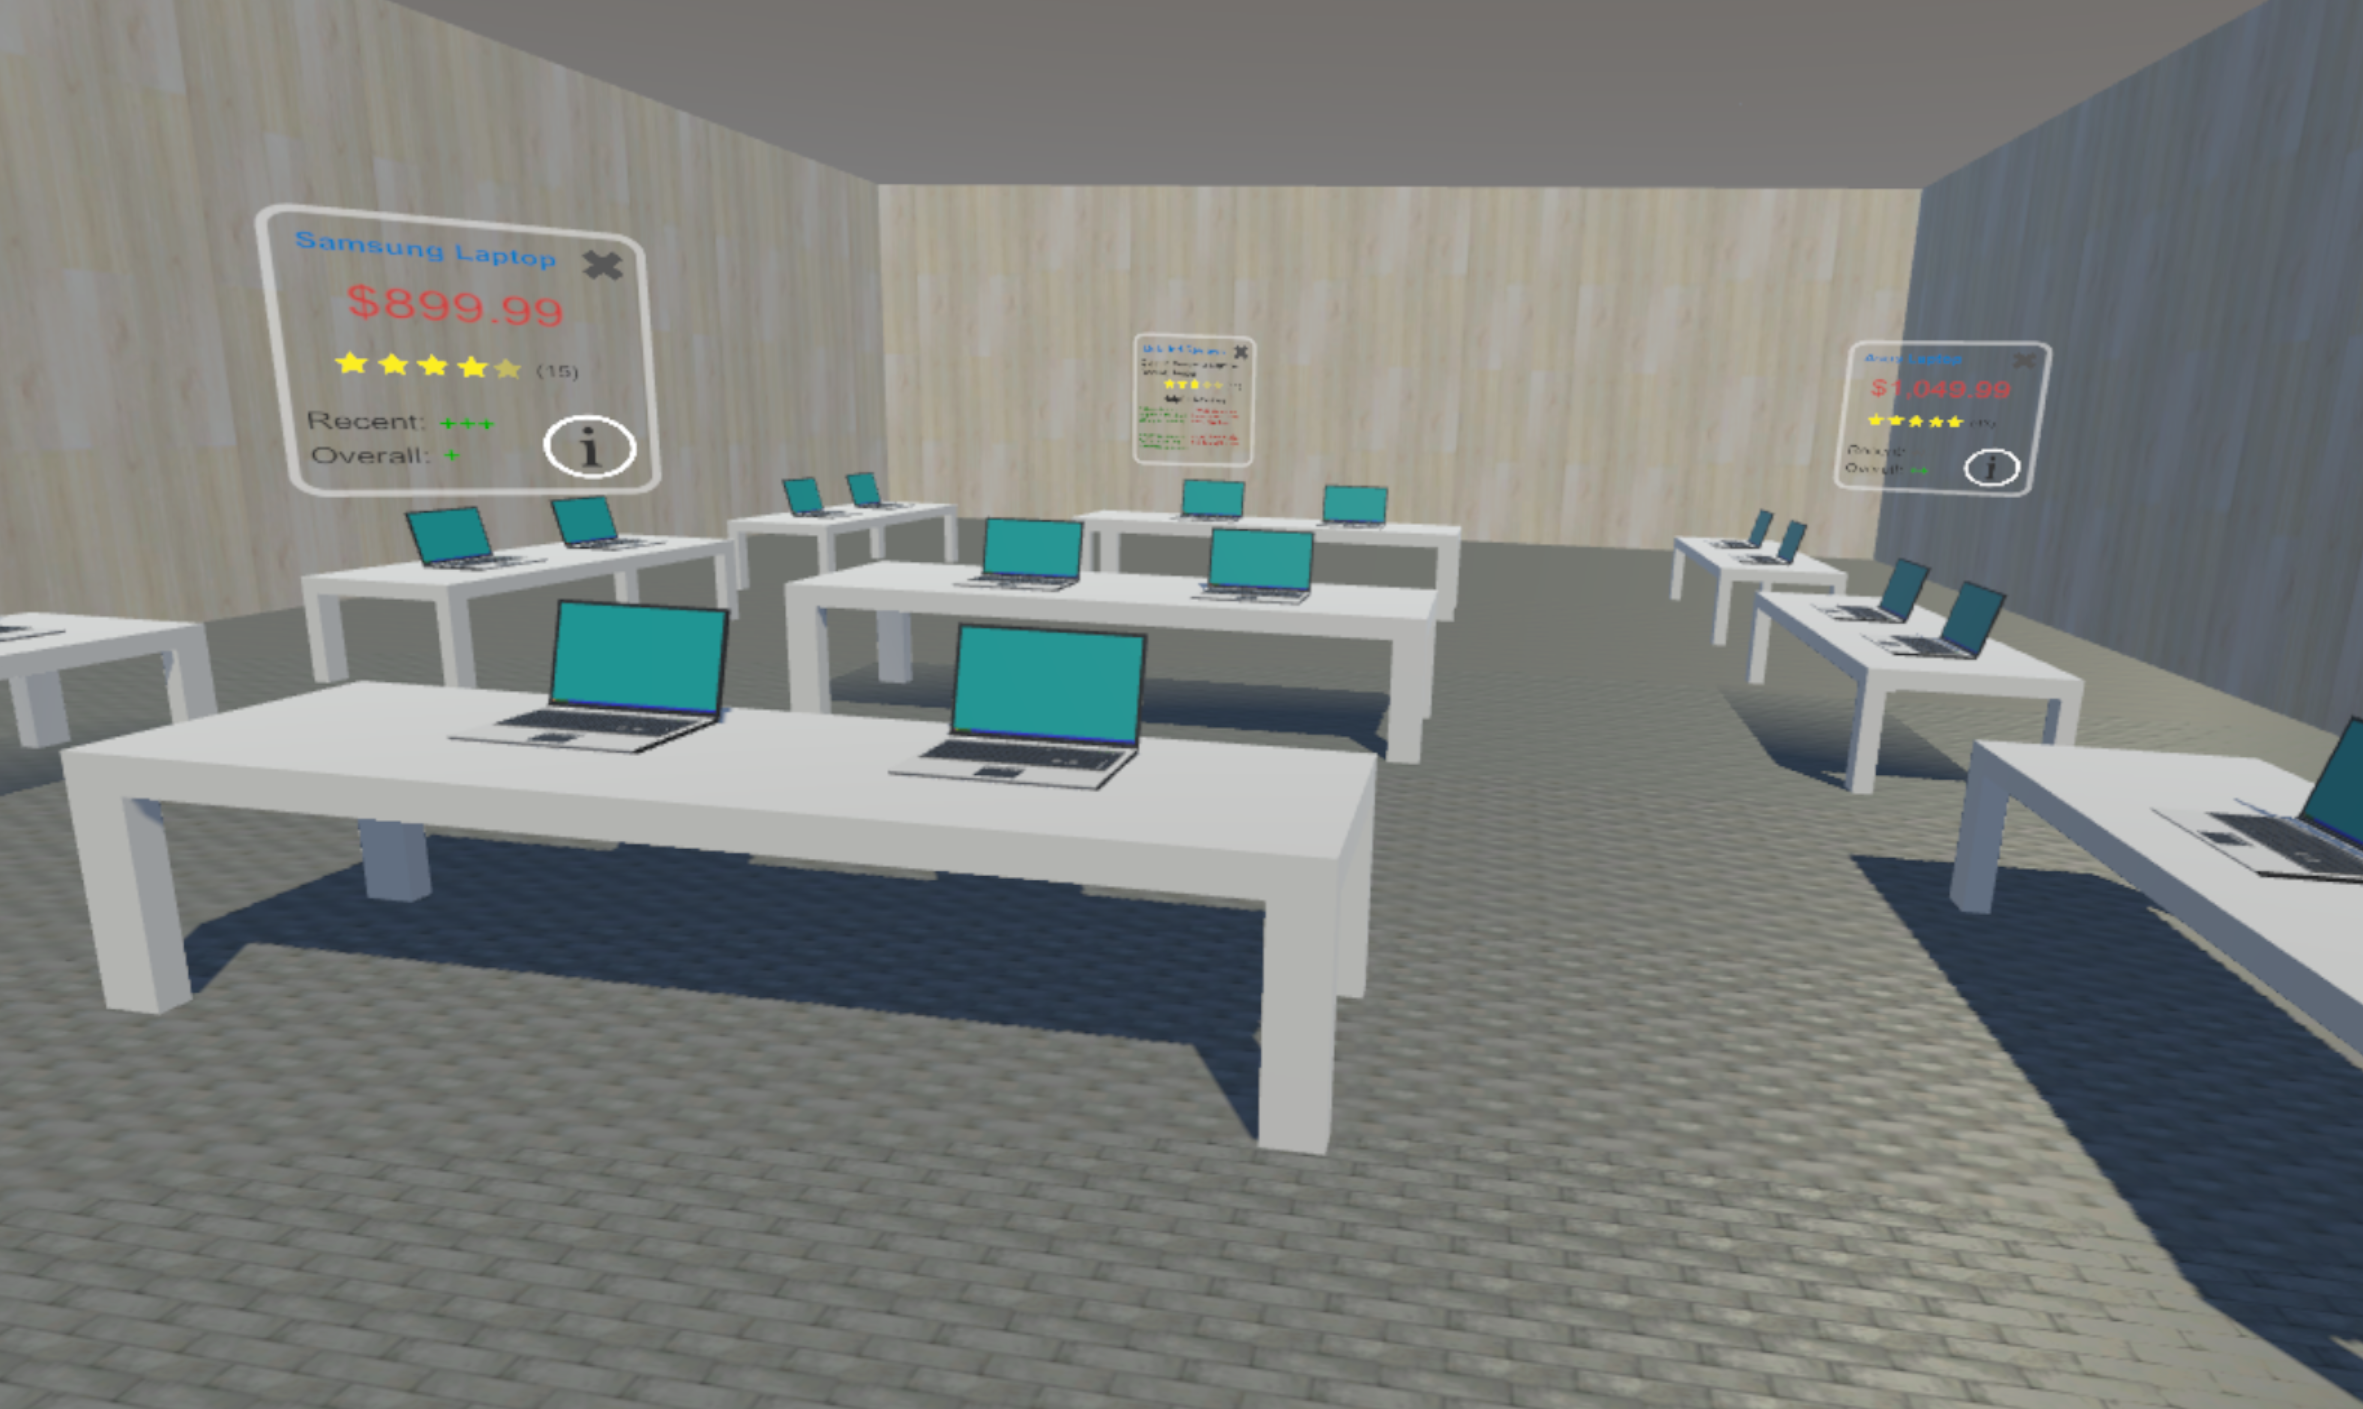
\includegraphics[width=0.9\columnwidth]{figures/3Panel}}
		\vfill
		\subfloat[][]{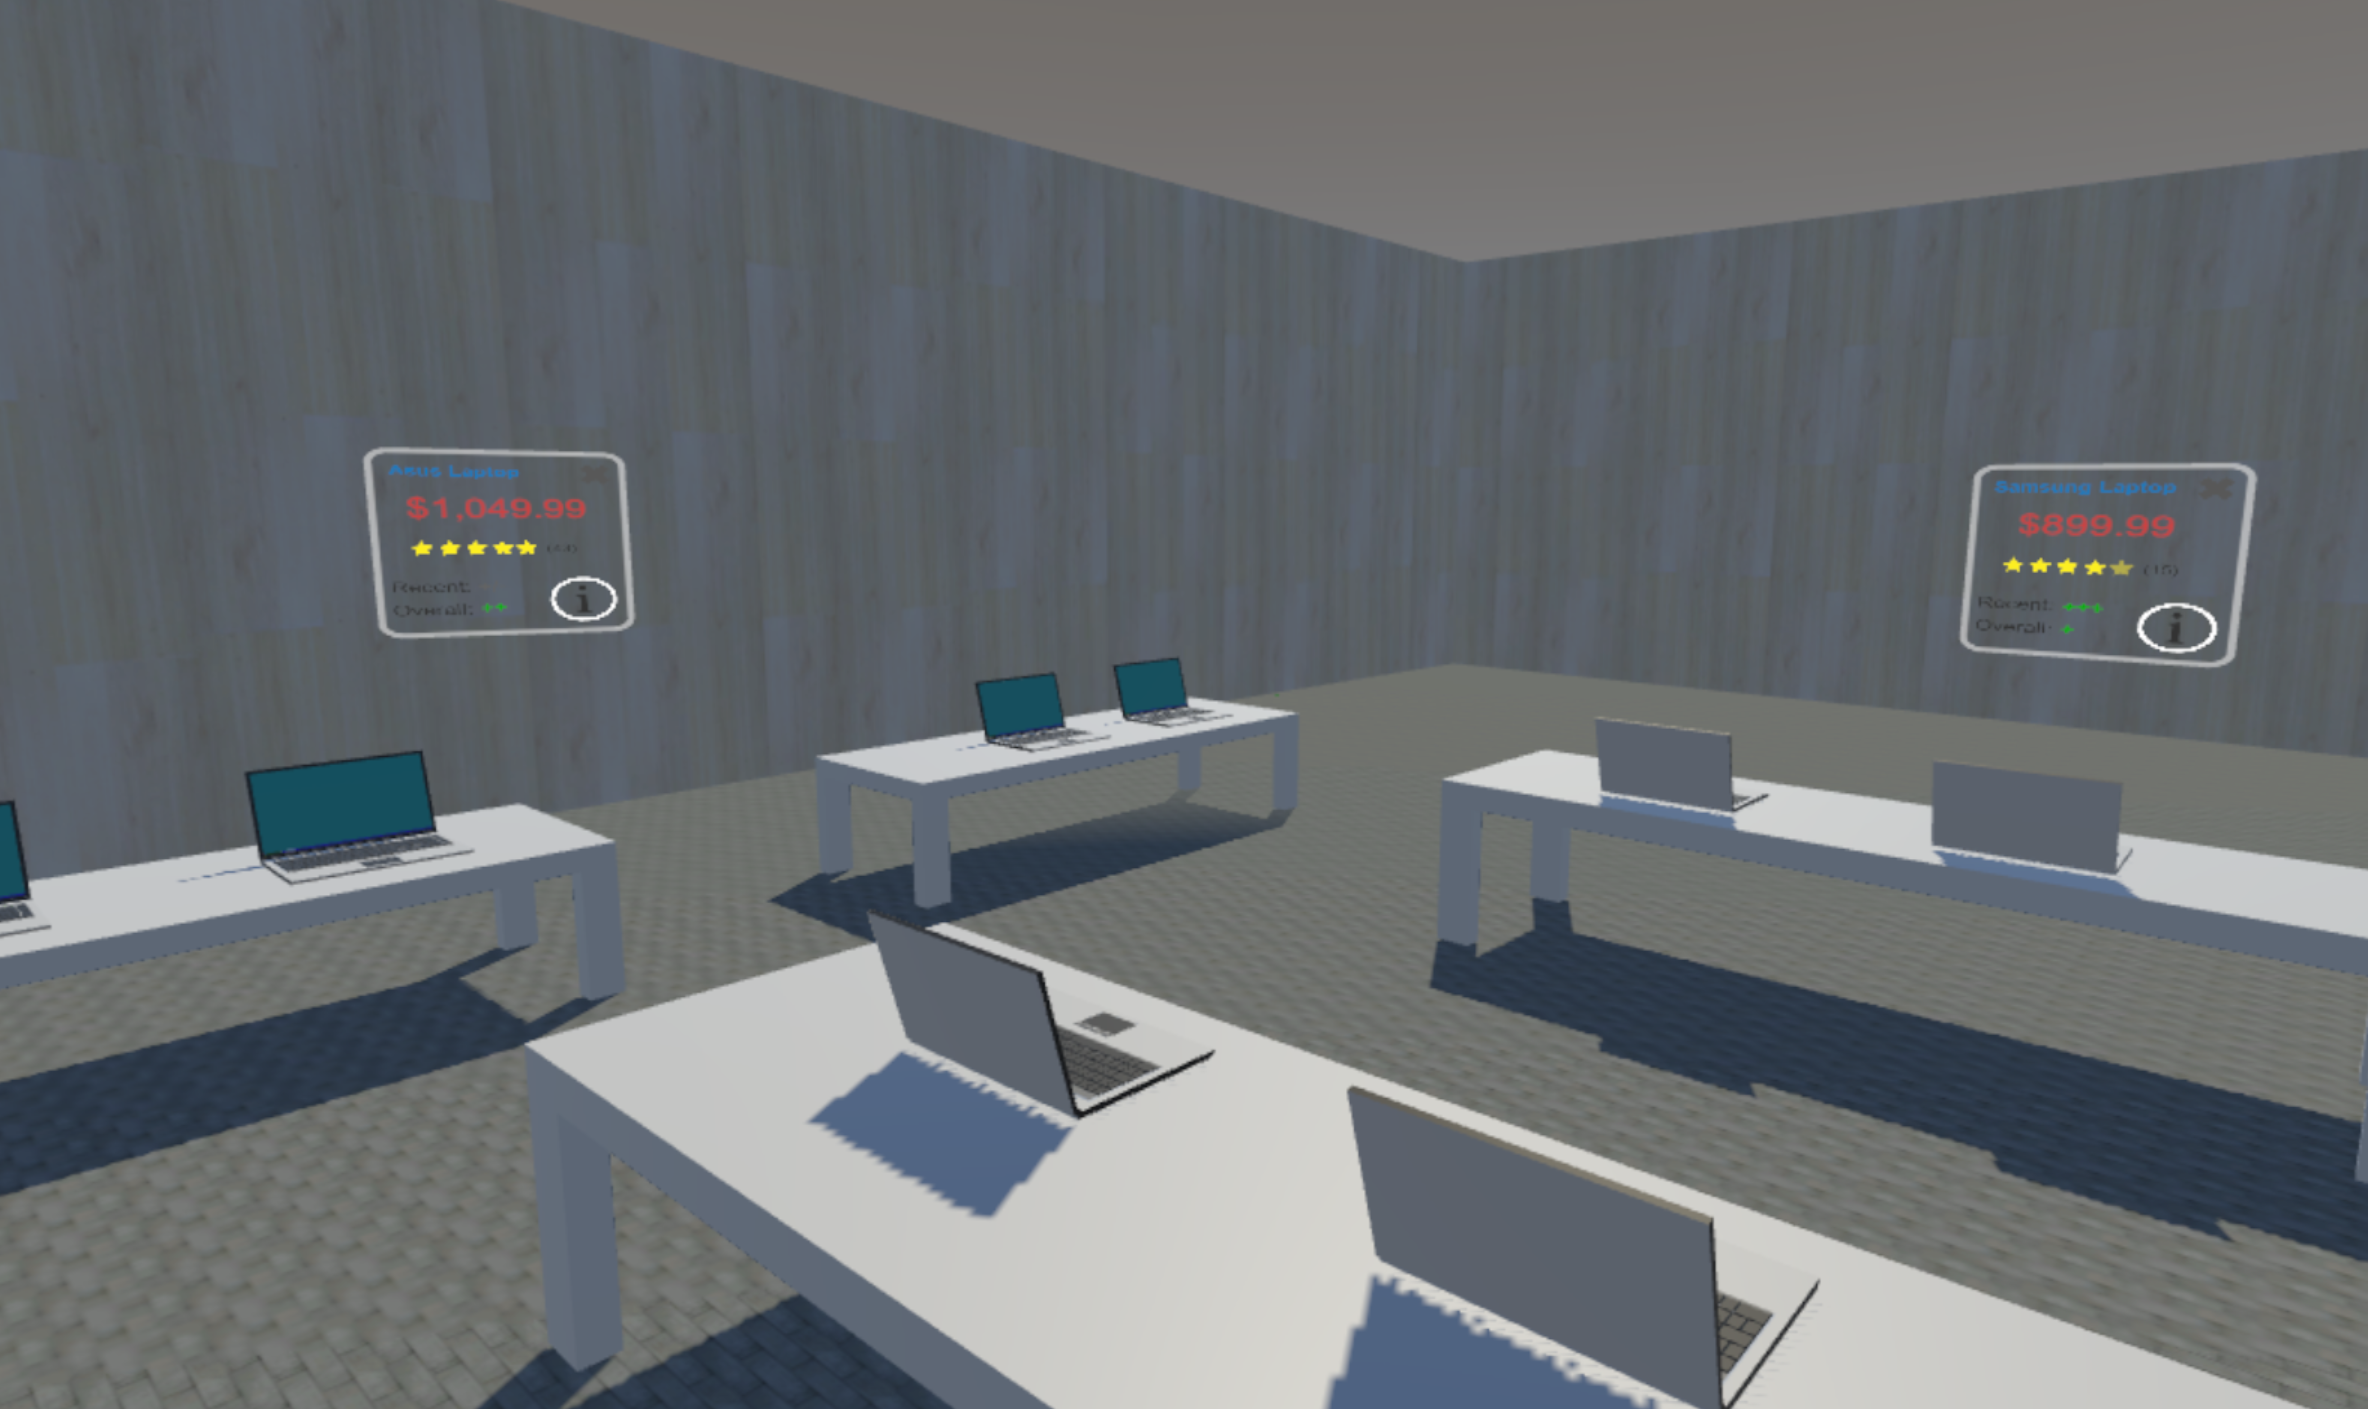
\includegraphics[width=0.9\columnwidth]{figures/2Panel}}
		\vfill
		\subfloat[][]{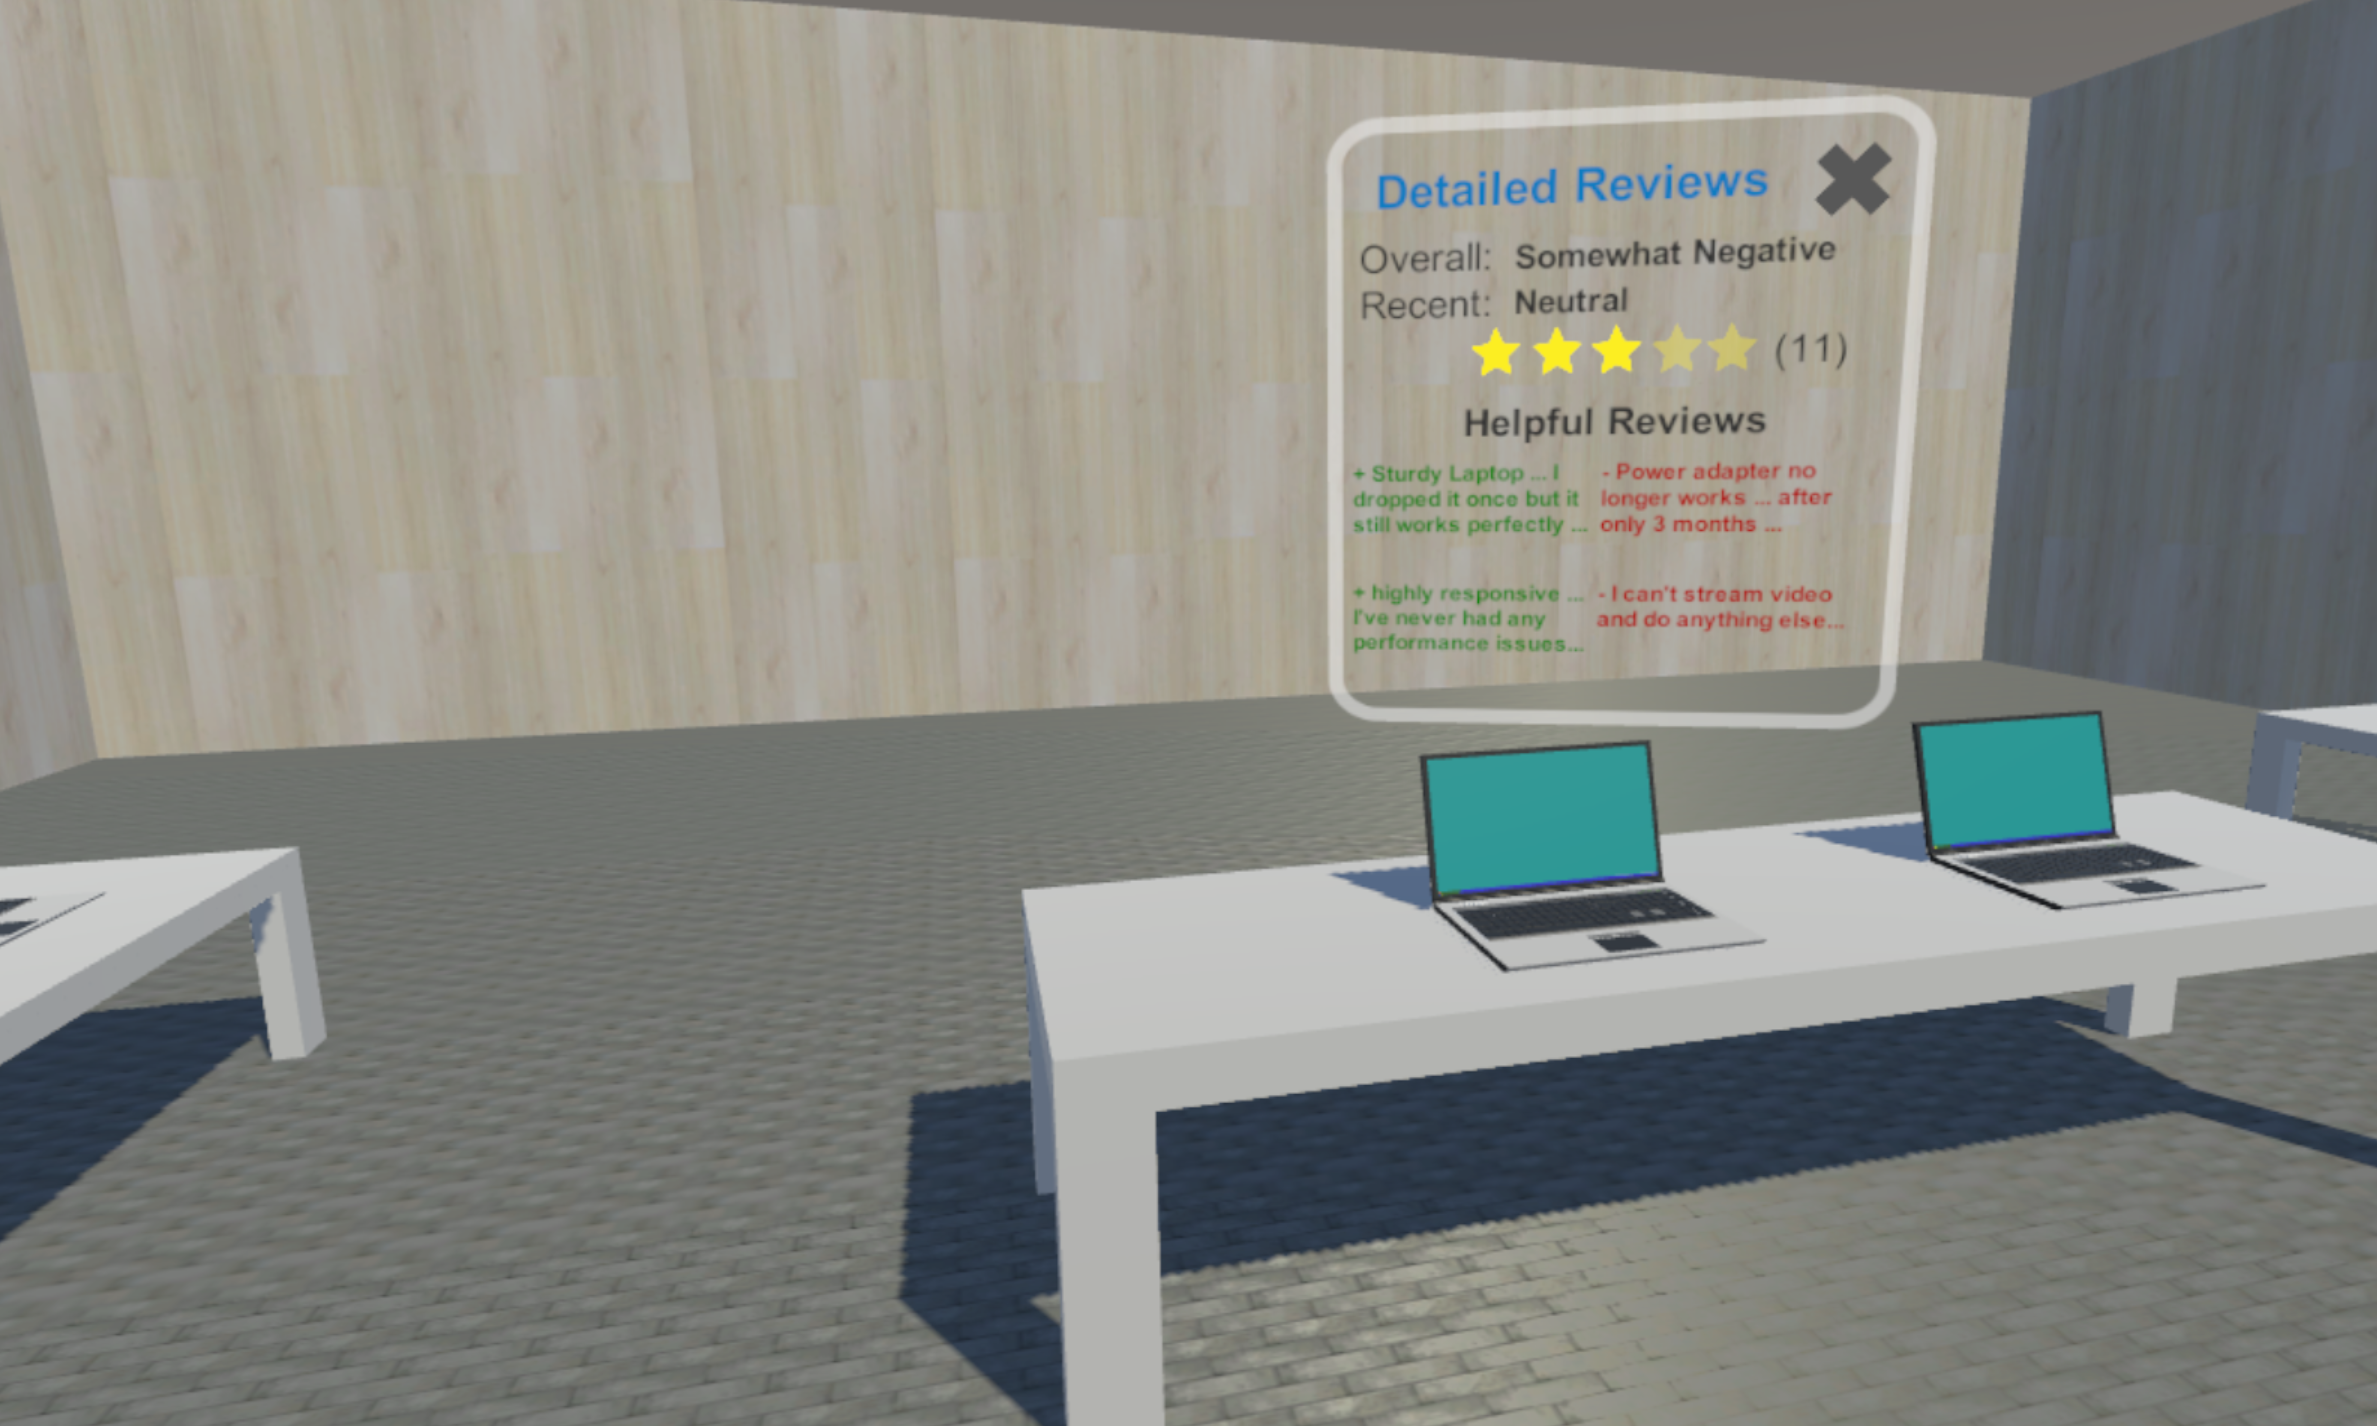
\includegraphics[width=0.9\columnwidth]{figures/DetailReviews}}
		\caption{In Phase Three, we designed an immersive simulated retail environment augmented with supplemental AR menus. We then measured participant responses to this StoAR prototype to provide preliminary data about what aspects of an augmented shopping experience might best support consumer decision making. \textbf{DNS: Please revise this wording :-)} }\label{figures:HiFiScreenshots}
	\end{minipage}
\end{marginfigure}

Participants envisioned using this platform for comparison shopping; rapid access to reviews, prices, and product specifications; and for visual demonstrations of product use. However, participants also felt minimizing the amount of visual information was key for reducing potential distractions and for a more streamlined retail experience. 
%Aligning with this vision of the system, participants listed lower depth of information as an expected trade-off. Participants expressed concern about digital content distracting them from the physical environment. 
%Having presented them with laptops, we asked participants for what other products they 
%think % JRB: w/c? Thought?
%augmented reality could aid them in decision-making, with the results shown in figure . \todo{MW: Games, toys, furniture, and clothing.  Honestly, this finding doesn't really line up with anything else, unless we start drawing conclusions about "They said furniture because of potential for visualizations" or something like that. We have a figure if we want to keep this point.} 
%DNS: This is talked about in the previous and next paragraph, so removed for space and to focus this paragraph on findings. Feel free to revise there if you'd like, but I think mentioning it is enough here. 
%We prompted participants for additional features they would like to have in a retail augmented reality system. 
Participants also desired several novel interactions with the provided content, including the ability to keep information ``pinned'' within a single view for comparing non-proximal products and to compare prices of a product against other stores' prices on-demand. 

In open-ended responses, many participants commented on the utility of the system for decision making in other contexts, for example in situations with aesthetic considerations, such as home furniture purchases, and for ``flipping'' the in-store buying process by allowing online shoppers access to simulated products on-demand from anywhere. Additionally, while some participants were concerned with the form factor of the HMD, open-ended responses showed a preference for the passive-viewing and contextualized information presented through the HMD compared to using mobile phones to access online information about a product in-store. 

%Two themes remained constant throughout the design process. Comparison shopping was listed as an important aspect of the online shopping experience in Phase One, and in Phases Two \& Three, participants viewed comparison shopping as an affordance of this system. Similarly, participants mentioned product demonstrations in phases 2 and 3. Though not mentioned in feedback from phase 1, data from phases 2 and 3 suggests that demonstrations or visualizations would be an effective application of augmented reality in shopping.
%DNS: Killing this for space and b/c the discussion is next and covers much of this. Good ideas here: worth coming back to in a camera-ready. 

%\todo[inline]{JRB: Same comment as Phase 2. This is a list of what they told you. Can you take it one step further and tell us what this means? What are the implications of these comments? You said you did this -- "We explored how understanding the trade-offs of parallel physical and virtual experiences could inform mixed reality applications in the context of retail shopping." -- so tell me what the results of this phase told you about those trade-offs. DNS--Yes, please! Especially look how things evolved from the first phase until here. Also, for Phase 2 \& 3, the idea of new applications, such as Demos came up. Those should be brought up in the findings as evidence of consumer thinking evolving with the design prompts--a big win for this type of methodology.}